\documentclass[a4paper]{article}
\usepackage{fancyhdr}
\usepackage[usenames, dvipsnames]{xcolor}
\usepackage{graphicx,hyperref,amsmath,float,subfigure,soul}
\usepackage[top=3cm,bottom=3cm,left=3cm,right=3cm]{geometry}
\hypersetup{
	colorlinks,
	citecolor=black,
	filecolor=black,
	linkcolor=black,
	urlcolor=black
}
\newcommand{\HRule}{\rule{\linewidth}{0.5mm}}
\pagestyle{fancy}
\lfoot{\small \color{gray}Tom Peerdeman - 10266186}
\cfoot{\thepage}
\rfoot{\small \color{gray}Ren\'e Aparicio Sa\'ez - 10214054}
\lhead{\small \color{gray}Multithreaded Wave}
\begin{document}
	\begin{titlepage}
	\begin{center}
		\textsc{\Large Concurrency \& Parallel Programming}\\[0.5cm]
		\HRule \\[0,4cm]
		\textsc{\huge \bfseries Multithreaded Wave}
		\HRule \\[8cm]
		\begin{minipage}{0.4\textwidth}
			\begin{flushleft}\large
				\emph{Auteurs: Tom Peerdeman \& Ren\'e Aparicio Saez}\\
			\end{flushleft}
		\end{minipage}
		\begin{minipage}{0.4\textwidth}
			\begin{flushright}\large
			\emph{Datum: 09-11-2012\\\hspace{1cm}}\\
			\end{flushright}
		\end{minipage}
	\end{center}
	\end{titlepage}

  \section{Table with results}
    Test on DAS4 are run for i = 1.000.000 and t = 1.000.
    The amount of threads used to generate the waves is increased to meassure the
    difference in speed for the program.
    Each amount of threads is run 12 times. 
    The highest value and the lowest value is disregarded. 
    The remaining data is used to plot a graph.\\\\
    \begin{tabular}{|c | c | c | c | c | c | c | c |}
      \hline
      \multicolumn{4}{|c}{i = 1,000,000} & \multicolumn{4}{c|}{t = 1,000}\\
      \hline
      1 thread & 2 threads & 3 threads & 4 threads & 5 threads & 6 threads & 7 threads & 8 threads\\
      \hline
      \st{3.61657} & \st{1.68174} & 1.67706 & 0.967125 & \st{0.955026} & 0.707557 & 0.907312 & 0.681091\\
      \hline
      3.68809 & 1.69923 & 1.62901 & 0.952905 & 1.11722 & 0.783331 & 0.888922 & 0.677461\\
      \hline
      3.68735 & 1.68316 & 1.71819 & 0.946174 & 1.10978 & \st{0.802315} & \st{0.919069} & 0.652223\\
      \hline
      3.75564 & 1.71218 & 1.66693 & \st{0.92198} & 1.19389 & 0.722481 & 0.87717 & 0.736193\\
      \hline
      3.82117 & 1.70358 & 1.69521 & 0.951281 & 1.18303 & 0.791841 & 0.895334 & 0.656148\\
      \hline
      3.85017 & 1.69776 & 1.74229 & \st{1.28526} & 1.18654 & 0.69405 & 0.900644 & 0.661786\\
      \hline
      3.74723 & 1.70488 & 1.73762 & 0.972624 & \st{1.21719} & 0.794964 & 0.91415 & 0.666394\\
      \hline
      3.80248 & \st{1.71702} & 1.6256 & 0.9513 & 1.18918 & 0.746098 & 0.888725 & \st{0.951125}\\
      \hline
      3.79577 & 1.69529 & \st{1.85265} & 0.949003 & 1.16967 & 0.789424 & 0.894571 & 0.66652\\
      \hline
      3.86725 & 1.70905 & \st{1.45095} & 0.958044 & 1.17816 & 0.716474 & 0.899676 & 0.710156\\
      \hline
      \st{3.91954} & 1.70727 & 1.81612 & 0.964905 & 1.19274 & 0.733274 & \st{0.882675} & \st{0.640491}\\
      \hline
      3.87399 & 1.70378 & 1.82773 & 0.960786 & 1.20634 & \st{0.682611} & 0.8860616 & 0.669534\\
      \hline
      \multicolumn{8}{|l|}{Average of the remaining 10:}\\
      \hline
      3.788914 & 1.701978 & 1.713576 & 0.9564147 & 1.173655 & 0.7479494 & 0.89525656 & 0.6777506\\
      \hline
    \end{tabular}
    \begin{center}
      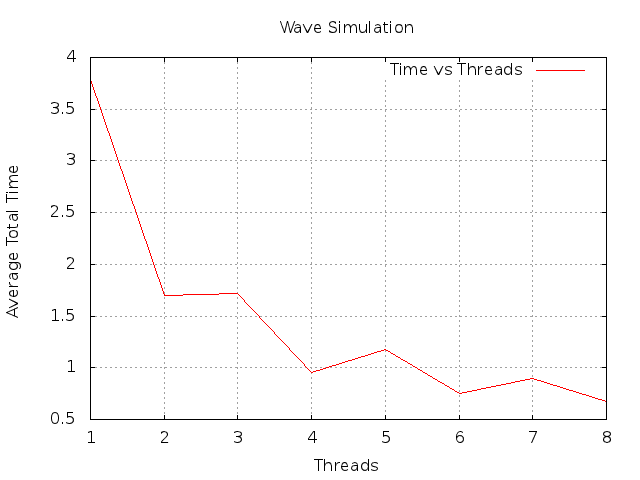
\includegraphics[width=0.9\textwidth]{speedplot.png}
    \end{center}
    Apparantly the preformance is better if an even number of threads is used.
\end{document}
